\refstepcounter{section}
\section*{Lecture 31: More on RG}
\addcontentsline{toc}{section}{Lecture 31: More on RG}
As a final thing, we will find the eigenvalues of the linearised RG matrix around the fixed point $\vb{K} = (\sfrac{1}{3},\sfrac{1}{9})$. Let us diagonalise the matrix, 
\begin{align*}
    \det(\mathrm{M}^{(\sqrt{2})} - \lambda \iden) = 0 \implies \det\mqty( \sfrac{4}{3}-\lambda & 1 \\ \sfrac{2}{3} & -\lambda )=0 \implies \lambda \qty(\lambda - \frac{4}{3}) =\frac{2}{3} \implies 3\lambda^2 - 4 \lambda -2 = 0
\end{align*}
which gives us $\lambda_\pm = \frac{1}{6}\qty(4\pm \sqrt{40}) \approx 1.7207, -0.3874$. Thus, $\abs{\lambda_+}>1$ and hence it is a \textit{relevant} eigenvalue, while $\abs{\lambda_+}<1$, rendering it \textit{irrelevant}. The corresponding eigenvectors are,
\begin{align*}
    \boldsymbol{u_+} =\mqty( 1\\ \frac{\sqrt{10}-2}{3} ) \approx  \mqty( 1\\ 0.387 )  \qquad  \boldsymbol{u_-} = \mqty(   1\\ -\frac{\sqrt{10}+2}{3} )  \approx \mqty( 1\\ -1.7207 ) 
\end{align*}
$\boldsymbol{u_+}$ is a relevant direction while $\boldsymbol{u_-}$ is an irrelevant direction which defines the critical surface.
Suppose we start initially at the point $(K_0,L_0)$ and successively apply the recursion formula. Upto linear approximation, we can expand the deviation $(K_0-K^*,L_0-L^*)$ in terms of the eigenvectors, that is, 
\begin{align}
    \mqty(K_0\\ L_0) = \mqty(K^*\\ L^*) + c_+ \boldsymbol{u_+} +c_-\boldsymbol{u_-} \quad \xrightarrow{l\ \text{transformations}} \quad \mqty(K_l\\ L_l) =\mqty(K^*\\ L^*) + \lambda_+^l c_+ \boldsymbol{u_+} +\lambda_-^l c_-\boldsymbol{u_-}
\end{align}
Now, suppose that after $l$ transformations, we want to reach the fixed point as much as possible. This cannot happen if $c_+$ is non-zero to begin with, as then, after the transformations, the deviation will grow along $u_+$. \\[0.2cm]
As an example, consider the original Ising model with nearest neighbour interaction only, that is, $L_0=0 $. We start from some $K_0 = K_c \neq 0$ and we have to take $c_+ = 0$ (since we want to go to the fixed point eventually). Then the above equation tells us, 
\begin{align*}
  \mqty(K_c\\ 0) = \mqty(\sfrac{1}{3}\\ \sfrac{1}{9}) + 0\cdot \boldsymbol{u_+} + c_-\mqty(   1\\ -\sfrac{\qty(\sqrt{10}+2)}{3} ) 
\end{align*} 
From which we obtain $c_-=\frac{1}{3\qty(2+\sqrt{10})}$ which implies $K_c = \frac{1}{3}+\frac{1}{3\qty(2+\sqrt{10})} \approx 0.3979$. This is the critical point for the nearest neighbour 2D Ising model, however, this is quite off from Onsager's exact solution $K_c = 0.4406$. Then starting from $(K_c,0)$ we will always go to the fixed point.
\begin{figure}[H]
    \centering
    

\tikzset{every picture/.style={line width=0.75pt}} %set default line width to 0.75pt        

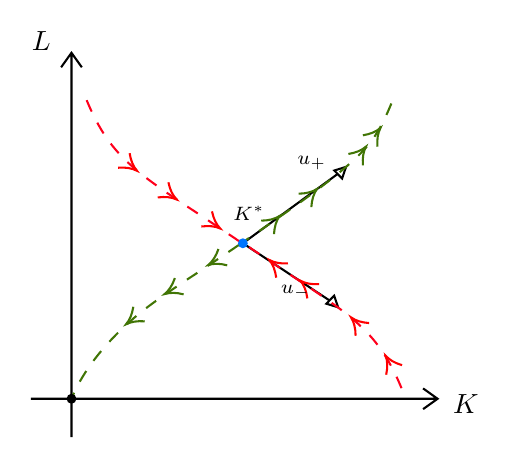
\begin{tikzpicture}[x=0.75pt,y=0.75pt,yscale=-1,xscale=1]
%uncomment if require: \path (0,300); %set diagram left start at 0, and has height of 300

%Straight Lines [id:da6968926015232697] 
\draw    (285.18,138.77) -- (333,103.8) ;
%Straight Lines [id:da2607102463275771] 
\draw    (285.18,138.77) -- (329.18,167.8) ;
%Shape: Axis 2D [id:dp25499887255247844] 
\draw [line width=0.75]  (183,213.69) -- (379,213.69)(202.6,47) -- (202.6,232.22) (372,208.69) -- (379,213.69) -- (372,218.69) (197.6,54) -- (202.6,47) -- (207.6,54)  ;
%Shape: Triangle [id:dp9819727702373128] 
\draw  [fill={rgb, 255:red, 255; green, 255; blue, 255 }  ,fill opacity=1 ] (334.89,101.96) -- (332.99,107.57) -- (329.23,103.72) -- cycle ;
%Shape: Triangle [id:dp4780886382683618] 
\draw  [fill={rgb, 255:red, 255; green, 255; blue, 255 }  ,fill opacity=1 ] (331.08,169.63) -- (325.41,167.9) -- (329.15,164.03) -- cycle ;
%Curve Lines [id:da8421690407171327] 
\draw [color={rgb, 255:red, 255; green, 0; blue, 28 }  ,draw opacity=1 ] [dash pattern={on 4.5pt off 4.5pt}]  (288.18,140.63) .. controls (312.35,157.09) and (327.77,166.38) .. (338.83,175.92) .. controls (349.19,184.87) and (355.71,194.03) .. (362,209.51) ;
%Shape: Boxed Bezier Curve [id:dp2633865727981807] 
\draw [color={rgb, 255:red, 255; green, 0; blue, 28 }  ,draw opacity=1 ] [dash pattern={on 4.5pt off 4.5pt}]  (283.36,137.77) .. controls (259.2,121.32) and (243.77,112.03) .. (232.72,102.49) .. controls (222.36,93.54) and (215.83,84.38) .. (209.54,68.9) ;
%Curve Lines [id:da788637893875605] 
\draw [color={rgb, 255:red, 65; green, 117; blue, 5 }  ,draw opacity=1 ] [dash pattern={on 4.5pt off 4.5pt}]  (283.18,139.63) .. controls (259.01,156.09) and (243.59,165.38) .. (232.54,174.92) .. controls (221.48,184.46) and (208.89,198.21) .. (202.6,213.69) ;
%Shape: Boxed Bezier Curve [id:dp9402772803574877] 
\draw [color={rgb, 255:red, 65; green, 117; blue, 5 }  ,draw opacity=1 ] [dash pattern={on 4.5pt off 4.5pt}]  (283.18,139.63) .. controls (307.35,123.18) and (323.83,111.5) .. (334.89,101.96) .. controls (345.94,92.42) and (350.71,86.24) .. (357,70.76) ;
%Shape: Ellipse [id:dp14907220449567005] 
\draw  [color={rgb, 255:red, 0; green, 115; blue, 255 }  ,draw opacity=1 ][fill={rgb, 255:red, 0; green, 118; blue, 255 }  ,fill opacity=1 ] (283.36,138.77) .. controls (283.36,137.75) and (284.18,136.91) .. (285.18,136.91) .. controls (286.19,136.91) and (287,137.75) .. (287,138.77) .. controls (287,139.8) and (286.19,140.63) .. (285.18,140.63) .. controls (284.18,140.63) and (283.36,139.8) .. (283.36,138.77) -- cycle ;
\draw  [color={rgb, 255:red, 255; green, 0; blue, 0 }  ,draw opacity=1 ] (230.62,95.38) .. controls (231.18,98.98) and (232.35,101.79) .. (234.14,103.84) .. controls (231.74,102.57) and (228.73,102.09) .. (225.1,102.38) ;
\draw  [color={rgb, 255:red, 255; green, 0; blue, 0 }  ,draw opacity=1 ] (249.3,109.41) .. controls (250.05,112.98) and (251.37,115.72) .. (253.27,117.66) .. controls (250.8,116.53) and (247.77,116.21) .. (244.16,116.7) ;
\draw  [color={rgb, 255:red, 255; green, 0; blue, 0 }  ,draw opacity=1 ] (270.3,123.41) .. controls (271.05,126.98) and (272.37,129.72) .. (274.27,131.66) .. controls (271.8,130.53) and (268.77,130.21) .. (265.16,130.7) ;
\draw  [color={rgb, 255:red, 255; green, 0; blue, 0 }  ,draw opacity=1 ] (361.88,197.5) .. controls (358.38,196.48) and (355.74,194.96) .. (353.95,192.93) .. controls (354.9,195.47) and (354.98,198.52) .. (354.23,202.08) ;
\draw  [color={rgb, 255:red, 255; green, 0; blue, 0 }  ,draw opacity=1 ] (345.99,177.22) .. controls (342.35,176.97) and (339.45,176.05) .. (337.26,174.44) .. controls (338.73,176.73) and (339.47,179.68) .. (339.49,183.33) ;
\draw  [color={rgb, 255:red, 65; green, 117; blue, 5 }  ,draw opacity=1 ] (336.02,95.74) .. controls (339.62,95.18) and (342.43,94.01) .. (344.48,92.22) .. controls (343.21,94.62) and (342.73,97.63) .. (343.02,101.26) ;
\draw  [color={rgb, 255:red, 65; green, 117; blue, 5 }  ,draw opacity=1 ] (312.03,114.88) .. controls (315.67,114.84) and (318.62,114.08) .. (320.9,112.6) .. controls (319.3,114.8) and (318.4,117.71) .. (318.17,121.35) ;
\draw  [color={rgb, 255:red, 65; green, 117; blue, 5 }  ,draw opacity=1 ] (294.03,127.88) .. controls (297.67,127.84) and (300.62,127.08) .. (302.9,125.6) .. controls (301.3,127.8) and (300.4,130.71) .. (300.17,134.35) ;
\draw  [color={rgb, 255:red, 65; green, 117; blue, 5 }  ,draw opacity=1 ] (343.02,86.74) .. controls (346.62,86.18) and (349.43,85.01) .. (351.48,83.22) .. controls (350.21,85.62) and (349.73,88.63) .. (350.02,92.26) ;
\draw  [color={rgb, 255:red, 65; green, 117; blue, 5 }  ,draw opacity=1 ] (273.41,141.54) .. controls (272.23,144.99) and (270.59,147.55) .. (268.48,149.25) .. controls (271.06,148.42) and (274.11,148.47) .. (277.63,149.39) ;
\draw  [color={rgb, 255:red, 65; green, 117; blue, 5 }  ,draw opacity=1 ] (252.41,155.54) .. controls (251.23,158.99) and (249.59,161.55) .. (247.48,163.25) .. controls (250.06,162.42) and (253.11,162.47) .. (256.63,163.39) ;
\draw  [color={rgb, 255:red, 65; green, 117; blue, 5 }  ,draw opacity=1 ] (232.39,169.38) .. controls (231.82,172.98) and (230.65,175.79) .. (228.86,177.83) .. controls (231.26,176.57) and (234.27,176.09) .. (237.9,176.39) ;
\draw  [color={rgb, 255:red, 255; green, 0; blue, 0 }  ,draw opacity=1 ] (321.92,158.47) .. controls (318.29,158.68) and (315.29,158.13) .. (312.92,156.81) .. controls (314.66,158.89) and (315.76,161.73) .. (316.24,165.34) ;
\draw  [color={rgb, 255:red, 255; green, 0; blue, 0 }  ,draw opacity=1 ] (306.92,148.47) .. controls (303.29,148.68) and (300.29,148.13) .. (297.92,146.81) .. controls (299.66,148.89) and (300.76,151.73) .. (301.24,155.34) ;
%Shape: Ellipse [id:dp5168078811686877] 
\draw  [color={rgb, 255:red, 0; green, 0; blue, 0 }  ,draw opacity=1 ][fill={rgb, 255:red, 0; green, 0; blue, 0 }  ,fill opacity=1 ] (200.78,213.69) .. controls (200.78,212.67) and (201.6,211.84) .. (202.6,211.84) .. controls (203.6,211.84) and (204.42,212.67) .. (204.42,213.69) .. controls (204.42,214.72) and (203.6,215.55) .. (202.6,215.55) .. controls (201.6,215.55) and (200.78,214.72) .. (200.78,213.69) -- cycle ;

% Text Node
\draw (279,119.4) node [anchor=north west][inner sep=0.75pt]  [font=\scriptsize]  {$K^{*}$};
% Text Node
\draw (302,157.4) node [anchor=north west][inner sep=0.75pt]  [font=\scriptsize]  {$u_{-}$};
% Text Node
\draw (310,95.4) node [anchor=north west][inner sep=0.75pt]  [font=\scriptsize]  {$u_{+}$};
% Text Node
\draw (385,210.4) node [anchor=north west][inner sep=0.75pt]    {$K$};
% Text Node
\draw (182,35.4) node [anchor=north west][inner sep=0.75pt]    {$L$};


\end{tikzpicture}

\end{figure}
\noindent 
Now, suppose we have $K_0\neq K_c$ which implies that, after $l$ transformations we no longer go to the fixed point.
\begin{figure}[H]
    \centering
  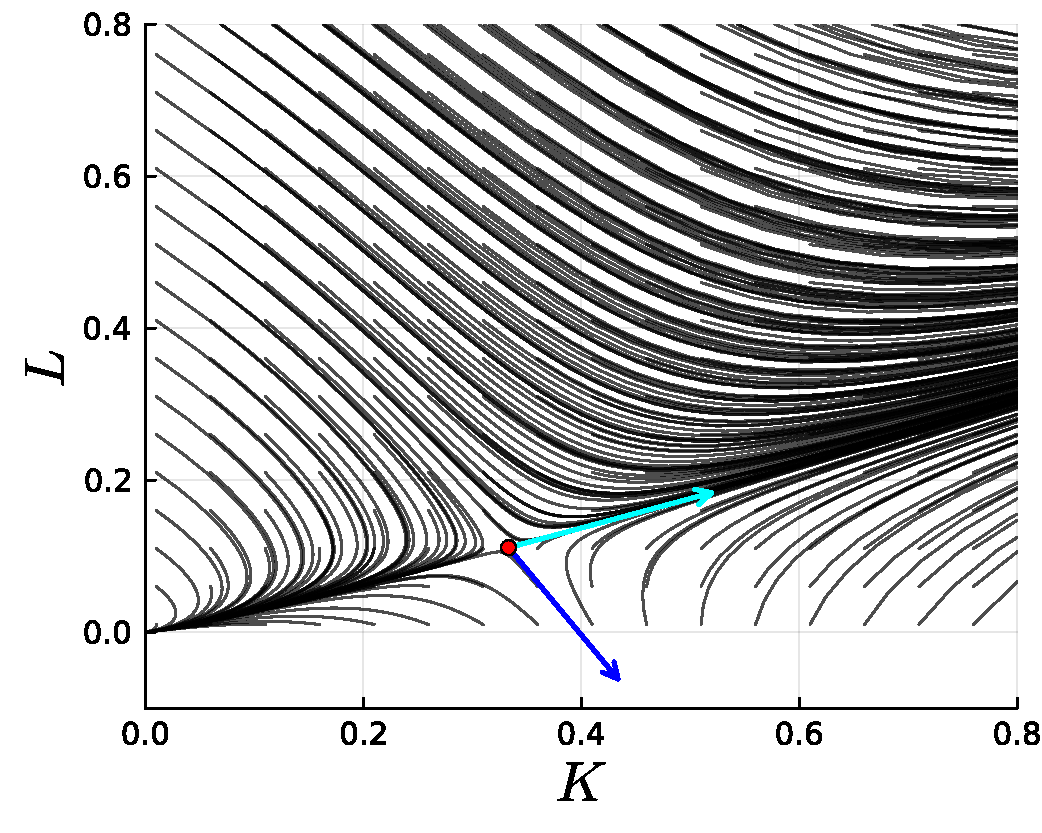
\includegraphics[width=0.6\textwidth]{codes/2D_Ising_RG.pdf}
\end{figure}